% latex uft-8
\documentclass[uplatex,a4paper,11pt,oneside,openany]{jsbook}
%
\usepackage[dvipdfmx]{graphicx}
\usepackage[dvipdfmx]{color}
\usepackage{amsmath,amssymb}
\usepackage{siunitx}
\usepackage{enumerate}
\usepackage{bm}
\usepackage{graphicx}
\usepackage{ascmac}
\usepackage{setspace}
\usepackage{here}
\usepackage{comment}
\usepackage{bm}
\usepackage{physics}
\usepackage{xcolor}
\usepackage{fancybox}
%\usepackage{jumoline}
\usepackage{listings,jlisting} %日本語のコメントアウトをする場合jlistingが必要
%ここからソースコードの表示に関する設定
\lstset{
	%プログラム言語(複数の言語に対応,C,C++も可)
 	language = Python,
 	%背景色と透過度
 	backgroundcolor={\color[gray]{.95}},
 	%枠外に行った時の自動改行
 	breaklines = true,
 	%自動改行後のインデント量(デフォルトでは20[pt])
 	breakindent = 10pt,
 	%標準の書体
 	%basicstyle = \ttfamily\scriptsize,
  basicstyle=\fontsize{8}{10}\selectfont\ttfamily,
 	%コメントの書体
 	commentstyle = {\itshape \color[cmyk]{1,0.4,1,0}},
 	%関数名等の色の設定
 	classoffset = 0,
 	%キーワード(int, ifなど)の書体
 	keywordstyle = {\bfseries \color[cmyk]{0,1,0,0}},
 	%表示する文字の書体
 	stringstyle = {\ttfamily \color[rgb]{0,0,1}},
 	%枠 "t"は上に線を記載, "T"は上に二重線を記載
	%他オプション:leftline,topline,bottomline,lines,single,shadowbox
 	frame = TBrl,
 	%frameまでの間隔(行番号とプログラムの間)
 	framesep = 5pt,
 	%行番号の位置
 	numbers = left,
	%行番号の間隔
 	stepnumber = 1,
	%行番号の書体
 	numberstyle = \tiny,
	%タブの大きさ
 	tabsize = 4,
 	%キャプションの場所("tb"ならば上下両方に記載)
 	captionpos = t
}
%ここまでソースコードの表示に関する設定
%ここからソースコードの表示に関する設定
%\lstset{
%  basicstyle={\ttfamily},
%  identifierstyle={\small},
%  commentstyle={\smallitshape},
%  keywordstyle={\small\bfseries},
%  ndkeywordstyle={\small},
%  stringstyle={\small\ttfamily},
%  frame={tb},
%  breaklines=true,
%  columns=[l]{fullflexible},
%  numbers=left,
%  xrightmargin=0zw,
%  xleftmargin=3zw,
%  numberstyle={\scriptsize},
%  stepnumber=1,
%  numbersep=1zw,
%  lineskip=-0.5ex
%}

\definecolor{mygreen}{rgb}{0,0.6,0}
\definecolor{mygray}{rgb}{0.5,0.5,0.5}
\definecolor{mymauve}{rgb}{0.58,0,0.82}

\lstdefinestyle{custompy}{
  belowcaptionskip=1\baselineskip,
  breaklines=true,
  numbers=left,
  frame=trBL,
  xleftmargin=\parindent,
  language=python,
  showstringspaces=false,
  basicstyle=\footnotesize\ttfamily,
  keywordstyle=\bfseries\color{green!40!black},
  commentstyle=\itshape\color{purple!40!black},
  %identifierstyle=\color{blue},
  %stringstyle=\color{orange},
  identifierstyle=\color{black},
  stringstyle=\color{black},
}
%ここまでソースコードの表示に関する設定
\makeatletter
\def\ps@plainfoot{%
  \let\@mkboth\@gobbletwo
  \let\@oddhead\@empty
  \def\@oddfoot{\normalfont\hfil-- \thepage\ --\hfil}%
  \let\@evenhead\@empty
  \let\@evenfoot\@oddfoot}
  \let\ps@plain\ps@plainfoot
\renewcommand{\chapter}{%
  \if@openright\cleardoublepage\else\clearpage\fi
  \global\@topnum\z@
  \secdef\@chapter\@schapter}
\makeatother
%
\newcommand{\maru}[1]{{\ooalign{%
\hfil\hbox{$\bigcirc$}\hfil\crcr%
\hfil\hbox{#1}\hfil}}}
%
\setlength{\textwidth}{\fullwidth}
\setlength{\textheight}{40\baselineskip}
\addtolength{\textheight}{\topskip}
\setlength{\voffset}{-0.55in}
%
\begin{document}
% START DOCUMENT
%
% COVER
\begin{center}
  \huge \par
  \vspace{15mm}
  \huge 2020\par
  \vspace{15mm}
  \LARGE Pendulum\par
  \vspace{100mm}
  \Large \date \par
  \vspace{15mm}
  \Large S.Matoike \par
  \vspace{10mm}
  \Large \par
  \vspace{10mm}
\end{center}
\thispagestyle{empty}
\clearpage
\addtocounter{page}{-1}
\newpage
\setcounter{tocdepth}{3}
%
\tableofcontents
%
%\chapter{はじめに}
\chapter{単振子}

\section{モデルの定式化}

%\begin{comment}
\begin{figure}[htbp]
  \begin{minipage}[b]{0.45\linewidth}
    \centering
    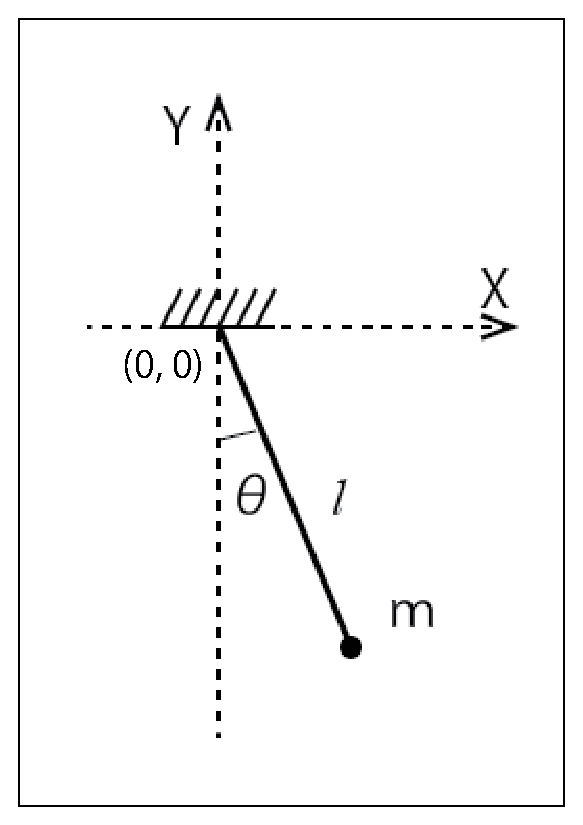
\includegraphics[keepaspectratio, scale=0.6]{eps/single.eps}
    \caption{単振子}
  \end{minipage}
  %\begin{minipage}[b]{0.45\linewidth}
    %\centering
    %\includegraphics[keepaspectratio, scale=0.35]{p13-2.eps}
    %\caption{p13-2}
  %\end{minipage}
\end{figure}
%\end{comment}

一方の端が固定され,質量を無視できる長さ$l$の棒の他端に,質量$m$の質点が拘束されている.棒が鉛直となす角は$\theta$,重力加速度は$g$である.

\[
\displaystyle T=\frac{1}{2}m(l\dot{\theta})^2,\quad U=-mgl\cos\theta
\]

より,Lagrangian$L=T-U$は,

\[
\displaystyle L=\frac{1}{2}ml^2\dot{\theta}^2+mgl\cos\theta
\]

Euler-Lagrange eq.は、

\[
\displaystyle\frac{\mathrm{d}}{dt}\frac{\partial L}{\partial \dot{\theta}}-\frac{\partial L}{\partial \theta}=0
\]

により次の通り.

\[
\displaystyle\ddot{\theta}=-\frac{g}{l}\sin\theta
\]

\section{Pythonで模擬実験}

これを次のように1階まで分解し,連立にして関数odeを定義する.\\

\begin{align*}
\displaystyle\frac{\mathrm{d}\theta}{\mathrm{d}t}&=\dot{\theta}\\\\
\displaystyle\frac{\mathrm{d}\dot{\theta}}{\mathrm{d}t}&=-\displaystyle\frac{g}{l}\sin\theta
\end{align*}\\

常微分方程式(Ordinary Differential Equation;ODE)の積分は,scipy.integrateのodeintを使う.関数odeの戻り値は,$[\theta,\dot{\theta}]$である.Pythonのアニメーションには,FuncAnimationを使う.

\lstset{escapechar=@,style=custompy}
\lstinputlisting[caption=単振子,label=pythonProgram1]{py/single.py}
 %single pendulum
\chapter{2重平面振子}

ランダウ、リフシッツ「力学」p13問題1(図1)

\section{モデルの定式化}

%\begin{comment}
\begin{figure}[htbp]
  \begin{minipage}[b]{0.45\linewidth}
    \centering
    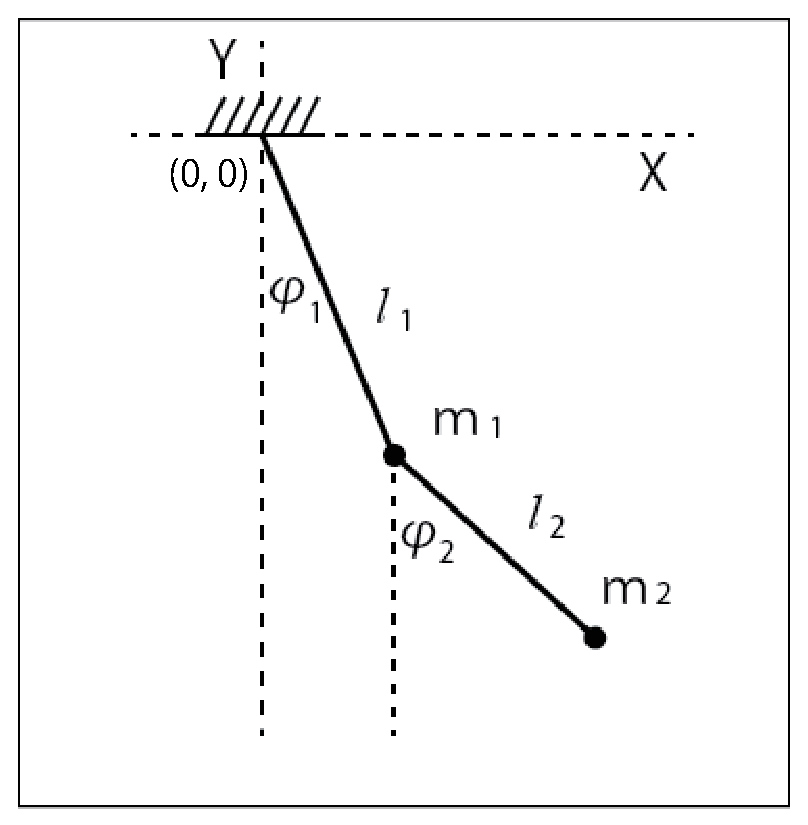
\includegraphics[keepaspectratio, scale=0.5]{eps/double.eps}
    \caption{2重平面振子}
  \end{minipage}
  %\begin{minipage}[b]{0.45\linewidth}
    %\centering
    %\includegraphics[keepaspectratio, scale=0.35]{p13-2.eps}
    %\caption{p13-2}
  %\end{minipage}
\end{figure}
%\end{comment}

棒$l_1$及び$l_2$が鉛直となす角を$\varphi_1,\varphi_2$とする.座標原点を支点におくことにすると, 質点の座標はそれぞれ

\[
(l_1\sin\varphi_1, -l_1\cos\varphi_1), \qquad (l_1\sin\varphi_1+l_2\sin\varphi_2, -l_1\cos\varphi_1-l_2\cos\varphi_2)
\]

質点$m_1$に対する運動エネルギー$T_1$,及びポテンシャル・エネルギー$U_1$は,

\[
\displaystyle T_1=\frac{1}{2}m_1(l_1\dot{\varphi_1})^2\quad,\qquad U_1=-m_1gl_1\cos\varphi_1
\]

($\displaystyle T_1=\frac{1}{2}m_1(\dot{x_1}^2+\dot{y_1}^2)$を計算しても,同じ結果になる.)\\

一方質点$m_2$について, そのデカルト座標$(x_2,y_2)$から,
\begin{align*}
x_2&=l_1\sin\varphi_1+l_2\sin\varphi_2\quad,\quad y_2=-(l_1\cos\varphi_1+l_2\cos\varphi_2)\\
\dot{x_2}&=l_1\dot{\varphi_1}\cos\varphi_1+l_2\dot{\varphi_2}\cos\varphi_2\quad,\quad\dot{y}_2=l_1\dot{\varphi_1}\sin\varphi_1+l_2\dot{\varphi_2}\sin\varphi_1\\
\dot{x}_2^2&=l_1^2\dot{\varphi_1}^2\cos^2\varphi_1+2l_1l_2\dot{\varphi_1}\dot{\varphi_2}\cos\varphi_1\cos\varphi_2+l_2^2\dot{\varphi_2}^2\cos^2\varphi_2\quad,\\
\dot{y}_2^2&=l_1^2\dot{\varphi_1}^2\sin^2\varphi_1+2l_1l_2\dot{\varphi_1}\dot{\varphi_2}\sin\varphi_1\sin\varphi_2+l_2^2\dot{\varphi_2}^2\sin^2\varphi_2
\end{align*}

運動エネルギーとポテンシャル・エネルギーは,\\
$\cos(\alpha-\beta)=\cos\alpha\cos\beta+\sin\alpha\sin\beta$,また $\sin^2\alpha+\cos^2\alpha=1$だから

\begin{align*}
\displaystyle T_2&=\frac{1}{2}m_2(\dot{x_2}^2+\dot{y_2}^2)=\frac{m_2}{2}\left(l_1^2\dot{\varphi_1}^2+l_2^2\dot{\varphi_2}^2+2l_1l_2\cos(\varphi_1-\varphi_2)\dot{\varphi_1}\dot{\varphi_2}\right)\\\\
U_2&=-m_2gl_1\cos\varphi_1-m_2gl_2\cos\varphi_2
\end{align*}

従って,Lagrangian$L=T_1+T_2-U_1-U_2$は,

\begin{align*}
L&=\displaystyle\frac{m_1+m_2}{2}l_1^2\dot{\varphi_1}^2+\frac{m_2}{2}l_2^2\dot{\varphi_2}^2+m_2l_1l_2\dot{\varphi_1}\dot{\varphi_2}\cos(\varphi_1-\varphi_2)\\\\
&\quad+(m_1+m_2)gl_1\cos\varphi_1+m_2gl_2\cos\varphi_2
\end{align*}

になる. 

\begin{align*}
\displaystyle\frac{\partial L}{\partial\varphi_1}&=-m_2l_1l_2\sin(\varphi_1-\varphi_2)\dot{\varphi_1}\dot{\varphi_2}-(m_1+m_2)gl_1\sin\varphi_1\quad,\\\\
\displaystyle\frac{\partial L}{\partial\dot{\varphi_1}}&=(m_1+m_2)l_1^2\dot{\varphi_1}+m_2l_1l_2\cos(\varphi_1-\varphi_2)\dot{\varphi_2}\quad,\\\\
\displaystyle\frac{\partial L}{\partial\varphi_2}&=m_2l_1l_2\sin(\varphi_1-\varphi_2)\dot{\varphi_1}\dot{\varphi_2}-m_2gl_2\sin\varphi_2\quad,\\\\
\displaystyle\frac{\partial L}{\partial\dot{\varphi_2}}&=m_2l_2^2\dot{\varphi_2}+m_2l_1l_2\cos(\varphi_1-\varphi_2)\dot{\varphi_1}
\end{align*}

より, Euler-Lagrange eq.

\[
\displaystyle \frac{\mathrm{d}}{\mathrm{d}t}\frac{\partial L}{\partial \dot{\varphi_i}}-\frac{\partial L}{\partial \varphi_i}=0
\]

は,

\begin{align*}
(m_1+m_2)l_1^2\ddot{\varphi_1}+m_2l_1l_2\cos(\varphi_1-\varphi_2)\ddot{\varphi_2}+m_2l_1l_2\sin(\varphi_1-\varphi_2)\dot{\varphi_1}\dot{\varphi_2}+(m_1+m_2)gl_1\sin\varphi_1&=0,\\\\
m_2l_2^2\ddot{\varphi_2}+m_2l_1l_2\cos(\varphi_1-\varphi_2)\ddot{\varphi_1}-m_2l_1l_2\sin(\varphi_1-\varphi_2)\dot{\varphi_1}\dot{\varphi_2}+m_2gl_2\sin\varphi_2&=0
\end{align*}

\section{Pythonによる模擬実験}

連立の常微分方程式にして,関数odeを定義する.

\begin{align*}
\displaystyle\frac{\mathrm{d}\varphi_1}{\mathrm{d}t}&=\dot{\varphi_1}\\\\
\displaystyle\frac{\mathrm{d}\varphi_2}{\mathrm{d}t}&=\dot{\varphi_2}\\\\
\displaystyle\frac{\mathrm{d}\dot{\varphi_1}}{\mathrm{d}t}&=\frac{Mg\sin\varphi_1+m_2\sin H(l_1\cos H+l_2)\dot{\varphi_1}\dot{\varphi_2}-m_2g\cos H\sin\varphi_2}{-\left(Ml_1-m_2l_1\cos^2H\right)}\\\\
\displaystyle\frac{\mathrm{d}\dot{\varphi_2}}{\mathrm{d}t}&=\frac{Mg\cos H\sin\varphi_1+\sin H(Ml_1+m_2l_2\cos H)\dot{\varphi_1}\dot{\varphi_2}-Mg\sin\varphi_2}{Ml_2-m_2l_2\cos^2H}
\end{align*}

ここで, $H=\varphi_1-\varphi_2 ,\quad M=m_1+m_2$である.

単振子との違いは質点が2個あるので,関数odeの戻り値は,単振子のときに$\left[\varphi, \dot{\varphi}\right]$としていたのを,$\left[\varphi_1, \dot{\varphi_1}, \varphi_2, \dot{\varphi_2}\right]$とする.

積分は,scipy.integrateのodeintを,アニメーションは,matplotlib.animationのFuncAnimationを使う.

\lstset{escapechar=@,style=custompy}
\lstinputlisting[caption=2重平面振子,label=pythonProgram2]{py/double.py}
 %double pendulum
\chapter{支点が水平方向に可動な単振子}

\section{モデルの定式化}

%\begin{comment}
\begin{figure}[htbp]
  \begin{minipage}[b]{0.45\linewidth}
    \centering
    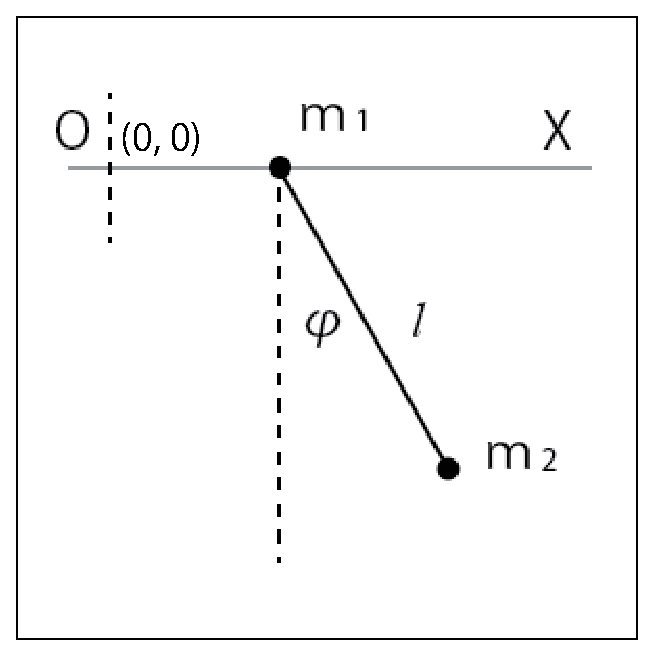
\includegraphics[keepaspectratio, scale=0.6]{movableh.eps}
    \caption{質量$m_1$の支点に質量$m_2$の単振子}
  \end{minipage}
  %\begin{minipage}[b]{0.45\linewidth}
    %\centering
    %\includegraphics[keepaspectratio, scale=0.35]{p13-2.eps}
    %\caption{p13-2}
  %\end{minipage}
\end{figure}
%\end{comment}

質量$m_2$の単振子.その支点である質量$m_1$の質点が水平方向に運動できる.

水平に運動している質点$m_1$の運動エネルギーは、

\[T_1 = \displaystyle\frac{m_1}{2}\dot{x}^2\]

質点$m_2$のデカルト座標$(x_2,y_2)$は、

\begin{align*}
   x_2 &= x + l\sin\varphi \quad,\quad y_2 = -l\cos\varphi\\
   \dot{x}_2 &= \dot{x} + l\dot{\varphi}\cos\varphi \quad,\quad \dot{y}_2 = l\dot{\varphi}\sin\varphi\\
   \dot{x}_2^2 &= \dot{x}^2 + 2\dot{x}l\dot{\varphi}\cos\varphi + l^2\dot{\varphi}^2\cos^2\varphi \quad,\quad \dot{y}_2^2 = l^2\dot{\varphi}^2\sin^2\varphi
\end{align*}

質点$m_2$の運動エネルギーは、$\sin^2\alpha+\cos^2\alpha=1$を思い出して、

\[T_2 = \displaystyle\frac{m_2}{2}\left(\dot{x}_2^2+\dot{y}_2^2\right) = \displaystyle\frac{m_2}{2}\left(\dot{x}^2 + 2l\dot{x}\dot{\varphi}\cos\varphi+l^2\dot{\varphi}^2\right)\]

一方、ポテンシャル・エネルギー$U$は、

\[U = -m_2gl\cos\varphi\]

従って、Lagrangian$L=T_1+T_2-U$は、

\[L=\displaystyle\frac{m_1+m_2}{2}\dot{x}^2+\frac{m_2}{2}\left(l^2\dot{\varphi}^2+2l\dot{x}\dot{\varphi}\cos\varphi\right)+m_2gl\cos\varphi\]

Euler-Lagrange eq.は,次の計算をして、

\begin{align*}
   \frac{\partial L}{\partial\dot{\varphi}}&=m_2l^2\dot{\varphi} + m_2l\dot{x}\cos\varphi \qquad,\quad \frac{\partial L}{\partial \varphi} = -m_2l\dot{x}\dot{\varphi}\sin\varphi - m_2gl\sin\varphi\\\\
   \frac{\partial L}{\partial \dot{x}} &= (m_1+m_2)\dot{x} + m_2l\dot{\varphi}\cos\varphi \qquad,\quad \frac{\partial L}{\partial x}=0
\end{align*}

従って,

\begin{align*}
   &m_2l^2\ddot{\varphi}-m_2l\dot{x}\sin\varphi = -m_2l\dot{x}\dot{\varphi}\sin\varphi - m_2gl\sin\varphi\\\\
   &\therefore \qquad \ddot{\varphi} = \frac{\sin\varphi}{l}\dot{x}+\frac{-\sin\varphi}{l}\dot{x}\dot{\varphi}+\frac{-g}{l}\sin\varphi
\end{align*}

もう一方の式は,

\begin{align*}
   &(m_1+m_2)\ddot{x}+m_2l\dot{\varphi}\cos\varphi=0\\\\
   &\therefore \qquad \ddot{x}=\displaystyle\frac{-m_2l\dot{\varphi}\cos\varphi}{m_1+m_2}
\end{align*}

\section{Pythonによる模擬実験}

これらを連立の一階微分方程式に直すと

\begin{align*}
   \displaystyle\frac{\mathrm{d}\varphi}{\mathrm{d}t}&=\dot{\varphi}\\\\
   \displaystyle\frac{\mathrm{d}x}{\mathrm{d}t}&=\dot{x}\\\\
   \displaystyle\frac{\mathrm{d}\dot{\varphi}}{\mathrm{d}t}&=\displaystyle\frac{\sin\varphi}{l}\dot{x}+\frac{-\sin\varphi}{l}\dot{x}\dot{\varphi}+\frac{-g}{l}\sin\varphi\\\\
   \displaystyle\frac{\mathrm{d}\dot{x}}{\mathrm{d}t}&=\displaystyle\frac{-m_2l\dot{\varphi}\cos\varphi}{m_1+m_2}
\end{align*}

2つの質点の座標$(x,y),(x_2,y_2)$については、座標$x$はラグランジアンに陽に含まれていないことから循環的な座標である.(ランダウ「力学」p.37)循環座標が存在する場合の運動方程式の積分は簡単化できて、$x$を含まない$L$を$x$で微分しても、その結果は定数(ゼロ)になる.

\[\displaystyle\frac{\mathrm{d}}{\mathrm{d}t}\frac{\partial L}{\partial \dot{x}}=\frac{\partial L}{\partial x}=0\]

時間微分$\displaystyle\frac{d}{dt}$の結果がゼロなので、$\displaystyle\frac{\partial L}{\partial\dot{x}}$は定数.

\[\displaystyle\frac{\partial L}{\partial \dot{x}}=(m_1+m_2)\dot{x}+m_2l\dot{\varphi}\cos\varphi=const.\]

これは系の運動量が保存することを表している.この式の積分は、
$(m_1+m_2)x + m_2l\sin\varphi = const.$,$const=0$に対して$x$が次の通り求まる.(ランダウ「力学」p.42 問3)

\begin{align*}
   x&=\frac{-m_2l\sin\varphi}{m_1+m_2}\\
   y&=0\\
   x_2&=x+l\sin\varphi\\
   y_2&=-y-l\cos\varphi
\end{align*}

支点の質量$m_1$を大きくして模擬実験を試すと、固定支点の状態に近づいてくる.($m_1\rightarrow\infty$で$x\rightarrow 0$,これは通常の単振子だ.)

\lstset{escapechar=@,style=custompy}
\lstinputlisting[caption=支点が水平方向に可動な単振子,label=pythonProgram3]{movableh.py}
 %horizontal movable
\chapter{支点が円周上を周回している単振子}

ランダウ、リフシッツ「力学」p13-14問題3(a)(図3)

p14に書かれているLagrangianの式は誤り。

\section{モデルの定式化}

%\begin{comment}
    \begin{figure}[htbp]
        \begin{minipage}[b]{0.45\linewidth}
          \centering
          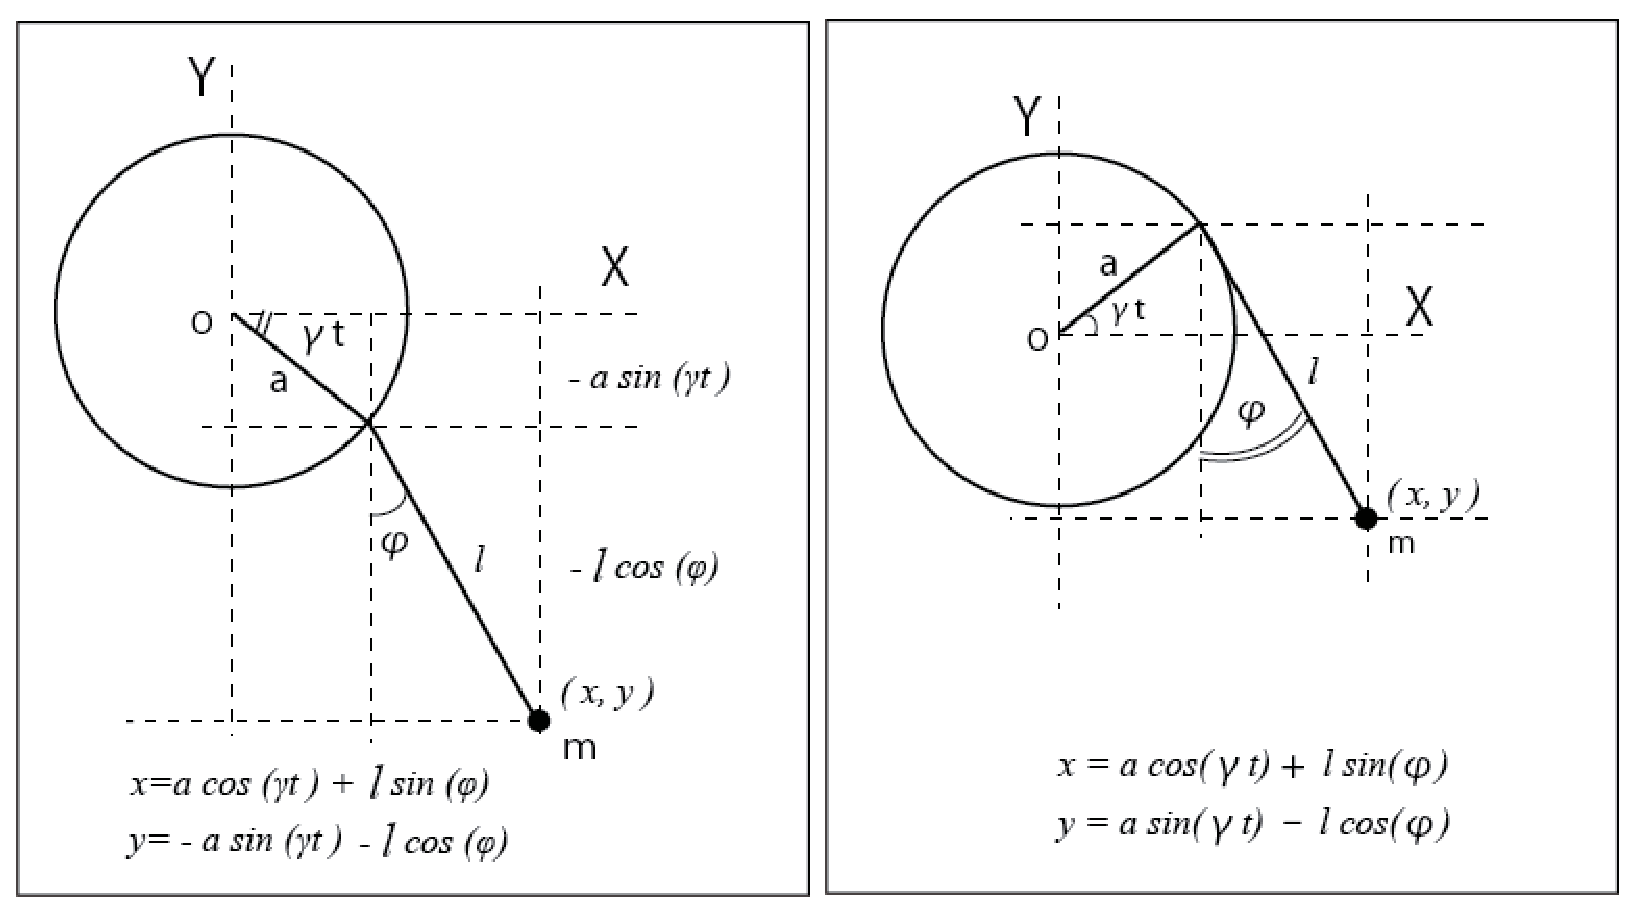
\includegraphics[keepaspectratio, scale=0.5]{eps/circular.eps}
          \caption{支点が円周上を周回する単振子}
        \end{minipage}
        %\begin{minipage}[b]{0.45\linewidth}
          %\centering
          %\includegraphics[keepaspectratio, scale=0.35]{p13-2.eps}
          %\caption{p13-2}
        %\end{minipage}
      \end{figure}
%\end{comment}

支点が鉛直平面内の円周上を一定の角速度$\gamma$で一様に動いている単振子. ($\gamma<0$でCW,$\gamma>0$でCCW,$\gamma$が$0$なら支点は動かない)

円周上の点に注目して($sin(-\gamma t)  = -sin(\gamma t)$だから)CWとCCWの違い

右の図は,CCW方向に回転する場合のモデル化になっている.質点$m$の位置$(x,y)$は,

\begin{align*}
   x&=a\cos\gamma t + l\sin\varphi\\
   y&=a\sin\gamma t - l\cos\varphi
\end{align*}

質点の速度,その自乗を作って,

\begin{align*}
   \dot{x}&=-a\gamma\sin\gamma t + l\dot{\varphi}\cos\varphi\\
   \dot{y}&=a\gamma\cos\gamma t + l\dot{\varphi}\sin\varphi\\
   \dot{x}^2&=a^2\gamma^2\sin^2\gamma t + l^2\dot{\varphi}^2\cos^2\varphi - 2al\gamma\dot{\varphi}\sin\gamma t\cos\varphi\\
   \dot{y}^2&=a^2\gamma^2\cos^2\gamma t + l^2\dot{\varphi}^2\sin^2\varphi + 2al\gamma\dot{\varphi}\sin\varphi\cos\gamma t
\end{align*}

運動エネルギー$T$とポテンシャル・エネルギー$U=mgy$は,

\begin{align*}
   T&=\displaystyle\frac{m}{2}\left(\dot{x}^2+\dot{y}^2\right)\\
   &=\frac{m}{2}\{a^2\gamma^2 + l^2\dot{\varphi}^2 + 2al\gamma\dot{\varphi}\left(\sin\varphi\cos\gamma t - \cos\varphi\sin\gamma t\right)\}\\
   &=\frac{m}{2}\{a^2\gamma^2 + l^2\dot{\varphi}^2 + 2al\gamma\dot{\varphi}\sin(\varphi-\gamma t)\}\\
   U&=mgy=mga\sin\gamma t - mgl\cos\varphi
\end{align*}

Lagrangian$L=T-U$は,

\begin{align*}
   L&=T-U\\
   &=\displaystyle\frac{m}{2}a^2\gamma^2 + \frac{m}{2}l^2\dot{\varphi}^2 + alm\gamma\dot{\varphi}\sin(\varphi-\gamma t) - mga\sin\gamma t + mgl\cos\varphi\\
   &=\frac{m}{2}l^2\dot{\varphi}^2 + alm\gamma\dot{\varphi}\sin(\varphi-\gamma t) + mgl\cos\varphi +\left(\frac{m}{2}a^2\gamma^2 - mga\sin\gamma t\right)
\end{align*}

右辺の最終項は, 次の関数$f(t)$の時間に関する完全導関数になっている.

\[f(t)=\displaystyle\frac{m}{2}a^2\gamma^2t + mga\frac{1}{\gamma}\cos\gamma t,\quad\frac{df(t)}{dt}=\frac{m}{2}a^2\gamma^2-mga\sin\gamma t\]

時間だけに依存する最終項を除けば,Lagrangianは最終的に次の様になる.(*座標と時間の任意の関数$f$の,時間に関する完全導関数$\dot{f}$をLagrangianの中に含んでいても,作用積分によってその変分は消えてしまう項になるので,取り除いても運動方程式としては変わらない.$\rightarrow$ランダウ「力学」p.5)

\[\therefore L=\displaystyle\frac{m}{2}l^2\dot{\varphi}^2 + alm\gamma\dot{\varphi}\sin(\varphi-\gamma t)+mgl\cos\varphi\]

次の計算をして,
\begin{align*}
   \displaystyle\frac{\partial L}{\partial\dot{\varphi}}&=ml^2\dot{\varphi} + alm\gamma\sin(\varphi-\gamma t)\\
   \displaystyle\frac{\partial L}{\partial\varphi}&=alm\gamma\dot{\varphi}\cos(\varphi-\gamma t)- mgl\sin\varphi
\end{align*}

もう少し準備して,

\[\displaystyle\frac{d}{dt}\frac{\partial L}{\partial\dot{\varphi}}=ml^2\ddot{\varphi}-alm\gamma^2\cos(\varphi-\gamma t)\]

Eular-Langange eq.

\[\displaystyle\frac{d}{dt}\frac{\partial L}{\partial\dot{\varphi}}-\frac{\partial L}{\partial\varphi}=0\]

は,

\[\therefore \ddot{\varphi}=\displaystyle\frac{a\gamma^2}{l}\cos(\varphi-\gamma t)+\frac{a\gamma}{l}\dot{\varphi}\cos(\varphi-\gamma t)-\frac{g}{l}\sin\varphi\]\\

一方, 左の図はCW方向に回転する場合のモデル化になっている.(実際, 右の図のモデルで$\gamma$を$-\gamma$で置き換えても同じ事になる.)質点$m$の位置$(x,y)$は,

\begin{align*}
   x&=a\cos\gamma t + l\sin\varphi\\
   y&=-a\sin\gamma t - l\cos\varphi
\end{align*}

質点の速度, その自乗と計算していくと,

\begin{align*}
   \dot{x}&=-a\gamma\sin\gamma t + l\dot{\varphi}\cos\varphi\\
   \dot{y}&=-a\gamma\cos\gamma t + l\dot{\varphi}\sin\varphi\\
   \dot{x}^2&=a^2\gamma^2\sin^2\gamma t + l^2\dot{\varphi}^2\cos^2\varphi - 2al\gamma\dot{\varphi}\sin\gamma t\cos\varphi\\
   \dot{y}^2&=a^2\gamma^2\cos^2\gamma t + l^2\dot{\varphi}^2\sin^2\varphi - 2al\gamma\dot{\varphi}\sin\varphi\cos\gamma t
\end{align*}

運動エネルギー$T$とポテンシャル・エネルギー$U$は,

\begin{align*}
   T&=\displaystyle\frac{m}{2}\left(\dot{x}^2+\dot{y}^2\right)\\
   &=\frac{m}{2}\{a^2\gamma^2 + l^2\dot{\varphi}^2 - 2al\gamma\dot{\varphi}\left(\sin\varphi\cos\gamma t + \cos\varphi\sin\gamma t\right)\}\\
   &=\frac{m}{2}\{a^2\gamma^2 + l^2\dot{\varphi}^2 - 2al\gamma\dot{\varphi}\sin(\varphi+\gamma t)\}\\
   U&=mgy= - mga\sin\gamma t - mgl\cos\varphi
\end{align*}

Lagrangian$L=T-U$は,

\begin{align*}
   L&=T-U\\&=\displaystyle\frac{m}{2}a^2\gamma^2 + \frac{m}{2}l^2\dot{\varphi}^2 - alm\gamma\dot{\varphi}\sin(\varphi+\gamma t) + mga\sin\gamma t + mgl\cos\varphi\\
   &=\frac{m}{2}l^2\dot{\varphi}^2 - alm\gamma\dot{\varphi}\sin(\varphi+\gamma t) + mgl\cos\varphi +\left(\frac{m}{2}a^2\gamma^2 + mga\sin\gamma t\right)
\end{align*}

右辺の最終項は, 次の関数$f(t)$の時間に関する完全導関数になっている.

\[f(t)=\displaystyle\frac{m}{2}a^2\gamma^2t - mga\frac{1}{\gamma}\cos\gamma t,\quad\frac{df(t)}{dt}=\frac{m}{2}a^2\gamma^2+mga\sin\gamma t\]

(*座標と時間の任意の関数$f$の,時間に関する完全導関数$\dot{f}$をLagrangianの中に含んでいても,作用積分によってその変分は消えてしまう項になるので,取り除いても運動方程式としては変わらない.$\rightarrow$ランダウ「力学」p.5)時間だけに依存する最終項を除けば,Lagrangianは最終的に次の様になる.

\[\therefore L=\displaystyle\frac{m}{2}l^2\dot{\varphi}^2 - alm\gamma\dot{\varphi}\sin(\varphi+\gamma t)+mgl\cos\varphi\]

次の計算をして,

\begin{align*}
   \displaystyle\frac{\partial L}{\partial\dot{\varphi}}&=ml^2\dot{\varphi} - alm\gamma\sin(\varphi+\gamma t)\\
   \displaystyle\frac{\partial L}{\partial\varphi}&=-alm\gamma\dot{\varphi}\cos(\varphi+\gamma t)- mgl\sin\varphi
\end{align*}

もう少し準備して,

\[\displaystyle\frac{d}{dt}\frac{\partial L}{\partial\dot{\varphi}}=ml^2\ddot{\varphi}-alm\gamma^2\cos(\varphi+\gamma t)\]

Eular-Langange eq.

\[\displaystyle\frac{d}{dt}\frac{\partial L}{\partial\dot{\varphi}}-\frac{\partial L}{\partial\varphi}=0\]

は,

\[\therefore \ddot{\varphi}=\displaystyle\frac{a\gamma^2}{l}\cos(\varphi+\gamma t)-\frac{a\gamma}{l}\dot{\varphi}\cos(\varphi+\gamma t)-\frac{g}{l}\sin\varphi\]

このCWの式は, CCWの場合のEular-Lgrange eq.の$\gamma$を$-\gamma$で置き換えて得られる式と同じ格好をしている.

\section{Pythonによる模擬実験}

連立の一階微分方程式に直して,関数ode定義する.右の図(CCWモデル)の場合のEular-Lagrange eq.からは,

\begin{align*}
   \displaystyle\frac{\mathrm{d}\varphi}{\mathrm{d}t}&=\dot{\varphi}\\\\
   \displaystyle\frac{\mathrm{d}\dot{\varphi}}{\mathrm{d}t}&=\displaystyle\frac{a\gamma^2}{l}\cos(\varphi-\gamma t) +\frac{a\gamma}{l}\dot{\varphi}\cos(\varphi-\gamma t)- \frac{g}{l}\sin\varphi
\end{align*}\\

円周上の点の位置$(x_0,y_0)$は、

\[x_0=a\cos\gamma t \quad,\quad y_0=a\sin\gamma t\]

であり、質点の位置$(x,y)$は、

\[x=x_0 + l\sin\varphi \qquad,\quad y=y_0 - l\cos\varphi\]

である.

左の図(CWモデル)の場合のEular-Lagrange eq.からは,

\begin{align*}
   \displaystyle\frac{\mathrm{d}\varphi}{\mathrm{d}t}&=\dot{\varphi}\\\\
   \displaystyle\frac{\mathrm{d}\dot{\varphi}}{\mathrm{d}t}&=\displaystyle\frac{a\gamma^2}{l}\cos(\varphi+\gamma t) -\frac{a\gamma}{l}\dot{\varphi}\cos(\varphi+\gamma t)- \frac{g}{l}\sin\varphi
\end{align*}

円周上の点の位置$(x_0,y_0)$は、

\[x_0=a\cos\gamma t \quad,\quad y_0=-a\sin\gamma t\]

であり、質点の位置$(x,y)$は、

\[x=x_0 + l\sin\varphi \qquad,\quad y=y_0 - l\cos\varphi\]

である.

模擬実験によって, CWとCCWの動きを確認することができる.わざわざ場合分けしてまでの記述をしているが, (当然の事ながら,) 一方の定式化だけにしておいて、定数GAMMAの符号を反転させても同じ現象になるよね.

\lstset{escapechar=@,style=custompy}
\lstinputlisting[caption=支点が円周上を周回する単振子,label=pythonProgram4]{py/circular.py}
 %circular moving
\chapter{支点が鉛直に振動している単振子}

ランダウ、リフシッツ「力学」p13-14問題3(c)

\section{モデルの定式化}

\begin{comment}
    \begin{figure}[htbp]
        \begin{minipage}[b]{0.45\linewidth}
          \centering
          \includegraphics[keepaspectratio, scale=0.6]{eps/vertical.eps}
          \caption{支点が鉛直に振動している単振子}
        \end{minipage}
        %\begin{minipage}[b]{0.45\linewidth}
          %\centering
          %\includegraphics[keepaspectratio, scale=0.35]{p13-2.eps}
          %\caption{p13-2}
        %\end{minipage}
      \end{figure}
\end{comment}

支点が鉛直方向に$a\cos\gamma t$にしたがって振動している単振子

単振子の座標は、$(l\sin\varphi,l\cos\varphi)$なので、質点$m$の座標は、$x= l\sin\varphi, y = a\cos\gamma t + l\cos\varphi$

次の準備をしておいて

\begin{align*}
   \dot{x} &= l\dot{\varphi}\cos\varphi \quad , \quad \dot{y}=-a\gamma\sin\gamma t - l\dot{\varphi}\sin\varphi\\
   \dot{x}^2 &= l^2\dot{\varphi}^2\cos^2\varphi \quad , \quad \dot{y}^2 = a^2\gamma^2\sin^2\gamma t +2a\gamma l \dot{\varphi}\sin\gamma t \sin\varphi + l^2\dot{\varphi}^2\sin^2\varphi
\end{align*}

運動エネルギー$T$とポテンシャル・エネルギー$U$は次の通り
($\sin^2\alpha+\cos^2\alpha=1$)

\begin{align*}
   T &= \frac{m}{2}\left(\dot{x}^2+\dot{y}^2\right)\\
   &=\frac{m}{2}\left(l^2\dot{\varphi}^2\left(\sin^2\varphi+\cos^2\varphi\right) +a^2\gamma^2\sin^2\gamma t + 2a\gamma l \dot{\varphi}\sin\gamma t\sin\varphi\right)\\
   &=\frac{m}{2}l^2\dot{\varphi}^2 + ma\gamma l\dot{\varphi}\sin\gamma t\sin\varphi + \frac{m}{2}a^2\gamma^2\sin^2\gamma t\\
   U &= -mgy\\&=-mg(a\cos\gamma t +l\cos\varphi)\\&=-mga\cos\gamma t - mgl\cos\varphi
\end{align*}

ラグランジアン$L=T-U$を求める.

\begin{align*}
   L &= T-U\\
   &=\frac{m}{2}l^2\dot{\varphi}^2 + ma\gamma l\dot{\varphi}\sin\gamma t\sin\varphi + \frac{m}{2}a^2\gamma^2\sin^2\gamma t + mga\cos\gamma t + mgl\cos\varphi\\
   &=\frac{m}{2}l^2\dot{\varphi}^2 +\left(ma\gamma^2l\cos\gamma t\cos\varphi -ma\gamma l\frac{d}{dt}(\cos\varphi\sin\gamma t)\right)\\
   &\qquad \qquad \qquad \qquad\quad \quad  +\frac{m}{2}a^2\gamma^2\sin^2\gamma t + mga\cos\gamma t +mgl\cos\varphi\\&=\frac{m}{2}l^2\dot{\varphi}^2+ma\gamma^2l\cos\gamma t\cos\varphi + mgl\cos\varphi\\
   &\qquad \qquad +\left(-ma\gamma l\frac{d}{dt}(\cos\varphi\sin\gamma t) + \frac{m}{2}a^2\gamma^2\sin^2\gamma t + mga\cos\gamma t \right)
\end{align*}

ここで、次の関係を使っている.
\begin{align*}
   -ma\gamma l\frac{d}{dt}(\cos\varphi\sin\gamma t) &= -ma\gamma l\left( -\dot{\varphi}\sin\varphi\sin\gamma t +\gamma\cos\varphi\cos\gamma t \right)\\
   &= ma\gamma l\dot{\varphi}\sin\gamma t\sin\varphi - ma\gamma^2l\cos\gamma t\cos\varphi
\end{align*}

更に、次の関数$f(\varphi,t)$を用意すると、

\[f(\varphi,t)=-ma\gamma l\cos\varphi\sin\gamma t + \displaystyle\frac{1}{4}ma^2\gamma^2t - \frac{1}{8}ma^2\gamma\sin 2\gamma t + mga\frac{1}{\gamma}\sin\gamma t\]

ラグランジアンの最後の括弧内の部分は、関数$f(\varphi,t)$の時間に関する完全導関数になっている.($\cos2\alpha=1-2\sin^2\alpha$)

\begin{align*}
   \frac{df(\varphi,t)}{dt}&=-ma\gamma l(-\dot{\varphi}\sin\varphi\sin\gamma t + \gamma\cos\varphi\cos\gamma t) +\frac{1}{4}ma^2\gamma^2 - \frac{1}{8}ma^2\gamma 2\gamma \cos2\gamma t + mga\frac{1}{\gamma}\gamma\cos\gamma t\\
   &= -ma\gamma l\frac{d}{dt}(\cos\varphi\sin\gamma t) + \frac{1}{4}ma^2\gamma^2 - \frac{1}{4}ma^2\gamma^2(1-2\sin^2\gamma t) + mga\cos\gamma t\\
   &= -ma\gamma l\frac{d}{dt}(\cos\varphi\sin\gamma t) + \frac{1}{4}ma^2\gamma^2 2\sin^2\gamma t + mga\cos\gamma t\\
   &= -ma\gamma l\frac{d}{dt}(\cos\varphi\sin\gamma t) + \frac{m}{2}a^2\gamma^2\sin^2\gamma t +mga\cos\gamma t
\end{align*}

従って、最終的なLagrangianは、(時間に関する完全導関数の部分を除いて)

\[L=\displaystyle\frac{ml^2}{2}\dot{\varphi}^2 + ma\gamma^2l\cos\gamma t\cos\varphi + mgl\cos\varphi\]

次の計算から

\begin{align*}
   \displaystyle\frac{\partial L}{\partial \dot{\varphi}}&=ml^2\dot{\varphi}\\
   \frac{\partial L}{\partial \varphi}&=-mla\gamma^2\cos\gamma t\sin\varphi -mgl\sin\varphi
\end{align*}

Euler-Lagrange eq.は

\begin{align*}
   \ddot{\varphi}=-\frac{a\gamma^2}{l}\cos\gamma t\sin\varphi - \frac{g}{l}\sin\varphi
\end{align*}

\section{Pythonによる模擬実験}

これを連立の一階微分方程式に直すと

\begin{align*}
   \frac{\mathrm{d}\varphi}{\mathrm{d}t} &= \dot{\varphi}\\
   \frac{\mathrm{d}\dot{\varphi}}{\mathrm{d}t} &= -\frac{a\gamma^2}{l}\cos\gamma t\sin\varphi - \frac{g}{l}\sin\varphi
\end{align*}

質点の座標は

\[x=l\sin\varphi \qquad,\quad y=a\cos\gamma t + l\cos\varphi\]

\lstset{escapechar=@,style=custompy}
\lstinputlisting[caption=支点が鉛直に振動している単振子,label=pythonProgram5]{py/vertical.py}
 %vertical
\chapter{支点が水平に振動している単振子}

\section{モデルの定式化}

\begin{comment}
    \begin{figure}[htbp]
        \begin{minipage}[b]{0.45\linewidth}
          \centering
          \includegraphics[keepaspectratio, scale=0.6]{horizontal.eps}
          \caption{支点が水平に振動している単振子}
        \end{minipage}
        %\begin{minipage}[b]{0.45\linewidth}
          %\centering
          %\includegraphics[keepaspectratio, scale=0.35]{p13-2.eps}
          %\caption{p13-2}
        %\end{minipage}
      \end{figure}
\end{comment}

単振子の座標は、$(l\sin\varphi,l\cos\varphi)$なので、質点$m$の座標は、

\[x=a\cos\gamma t + l\sin\varphi, y = l\cos\varphi\]

予め次の計算の準備をしておいて、

\begin{align*}
   \dot{x} &= -a\gamma\sin\gamma t +l\dot{\varphi}\cos\varphi \quad,\quad \dot{y} = -l\dot{\varphi}\sin\varphi\\
   \dot{x}^2 &= a^2\gamma^2\sin^2\gamma t - 2a\gamma l\dot{\varphi}\sin\gamma t\cos\varphi + l^2\dot{\varphi}^2\cos^2\varphi\quad,\quad \dot{y}^2 =l^2\dot{\varphi}^2\sin^2\varphi
\end{align*}

運動エネルギー$T$とポテンシャル・エネルギー$U$は次のようになる($\sin^2\alpha+\cos^2\alpha=1$を使って)

\begin{align*}
   T &= \frac{m}{2}(\dot{x}^2+\dot{y}^2)\\
   &=\frac{m}{2}l^2\dot{\varphi}^2\left(\sin^2\varphi+\cos^2\varphi\right) -ma\gamma l\dot{\varphi}\sin\gamma t\cos\varphi + \frac{m}{2}a^2\gamma^2\sin^2\gamma t\\
   &=\frac{m}{2}l^2\dot{\varphi}^2 -ma\gamma l\dot{\varphi}\sin\gamma t\cos\varphi + \frac{m}{2}a^2\gamma^2\sin^2\gamma t\\
   U &= -mgy = -mgl\cos\varphi
\end{align*}

ラグランジアン$ L=T-U $を求めていく.

\begin{align*}
   L &= T-U\\&=\frac{m}{2}l^2\dot{\varphi}^2 -ma\gamma l\dot{\varphi}\sin\gamma t\cos\varphi + \frac{m}{2}a^2\gamma^2\sin^2\gamma t + mgl\cos\varphi\\
   &= \frac{m}{2}l^2\dot{\varphi}^2 + \left(ma\gamma^2l \cos\gamma t\sin\varphi -ma\gamma l\frac{d}{dt}(\sin\varphi\sin\gamma t) \right) +\\
   &\qquad\qquad\qquad\qquad\qquad\qquad\qquad\qquad\frac{m}{2}a^2\gamma^2\sin^2\gamma t + mgl\cos\varphi\\
   &= \frac{m}{2}l^2\dot{\varphi}^2 +ma\gamma^2l \cos\gamma t\sin\varphi +\\&\qquad\qquad\left(-ma\gamma l\frac{d}{dt}(\sin\varphi\sin\gamma t)\frac{m}{2}a^2\gamma^2\sin^2\gamma t\right) +  mgl\cos\varphi
\end{align*}

ここで、次の関係を使っている.

\begin{align*}
   -ma\gamma l\frac{d}{dt}\left(\sin\varphi\sin\gamma t\right)&= -ma\gamma l\left(\gamma\sin\varphi\cos\gamma t +\dot{\varphi}\cos\varphi\sin\gamma t\right)\\
   &= -ma\gamma^2 l\sin\varphi\cos\gamma t - ma\gamma l\dot{\varphi}\cos\varphi\sin\gamma t
\end{align*}

更に、次の関数$f(\varphi,t)$を用意する、

\[f(\varphi,t) = -ma\gamma l\sin\varphi\sin\gamma t + \displaystyle\frac{1}{4}ma^2\gamma^2 t - \frac{1}{8}ma^2\gamma\sin 2\gamma t\]

ラグランジアンの最後の括弧内の部分は、関数$f(\varphi,t)$の時間に関する完全導関数になっている.($\cos 2\alpha=1-2\sin^2\alpha$を使って)

\begin{align*}
   \frac{df(\varphi,t)}{dt} &= -ma\gamma l\frac{d}{dt}(\sin\varphi\sin\gamma t) + \frac{1}{4}ma^2\gamma^2 - \frac{1}{8}ma^2\gamma(2\gamma)\cos 2\gamma t\\
   &= -ma\gamma l\frac{d}{dt}(\sin\varphi\sin\gamma t) + \frac{1}{4}ma^2\gamma^2 - \frac{1}{4}ma^2\gamma^2(1-2\sin^2\gamma t)\\&= -ma\gamma l\frac{d}{dt}(\sin\varphi\sin\gamma t) + \frac{1}{4}ma^2\gamma^2(2\sin^2\gamma t)\\
   &= -ma\gamma l\frac{d}{dt}(\sin\varphi\sin\gamma t) + \frac{m}{2}a^2\gamma^2\sin^2\gamma t
\end{align*}

従って、最終的なLagrangianは、(時間に関する完全導関数を除いて)

\[L=\displaystyle\frac{ml^2}{2}\dot{\varphi}^2+mla\gamma^2\cos\gamma t\sin\varphi + mgl\cos\varphi\]

次の計算から,

\begin{align*}
   \frac{\partial L}{\partial \dot{\varphi}} &= ml^2\dot{\varphi}\\
   \frac{\partial L}{\partial \varphi} &= mla\gamma^2\cos\gamma t\cos\varphi - mgl\sin\varphi
\end{align*}

Euler-Lagrange eq.は

\[\ddot{\varphi}=\displaystyle\frac{a\gamma^2}{l}\cos\gamma t\cos\varphi - \frac{g}{l}\sin\varphi\]

\section{Pythonによる模擬実験}

これを連立の一階微分方程式に直すと

\begin{align*}
   \frac{\mathrm{d}\varphi}{\mathrm{d}t} &= \dot{\varphi}\\
   \frac{\mathrm{d}\dot{\varphi}}{\mathrm{d}t} &= \frac{a\gamma^2}{l}\cos\gamma t\cos\varphi - \frac{g}{l}\sin\varphi
\end{align*}

質点の座標は

\[x=a\cos\gamma t + l\sin\varphi \qquad,\quad y=l\cos\varphi\]

\lstset{escapechar=@,style=custompy}
\lstinputlisting[caption=支点が水平に振動している単振子,label=pythonProgram6]{horizontal.py}
 %horizontal
%\chapter{おわりに}
\newpage
%
\section*{謝辞}
\addcontentsline{toc}{chapter}{謝辞}
%
\begin{thebibliography}{99}
  \bibitem{1}
\end{thebibliography}
%
% END DOCUMENT
\end{document}
%
